\chapter{Algorithm design} \label{ch:alganalysis}
This chapter will explore the algorithm domain in the A$^3$ model described in section \vref{sec:a3model} and it is the domain marked on figure \vref{fig:a3alg}. This chapter will describe the two stereo vision algorithms, \textit{Efficient Edge Preserving Stereo Matching} (EEPSM) and \textit{Fast Cost-Volume Matching} (FCV). Lastly, a simulation of each algorithm is created and the results of these simulations are compared and from this, an algorithm is chosen.\\

\begin{figure}[ht!]
  \centering
  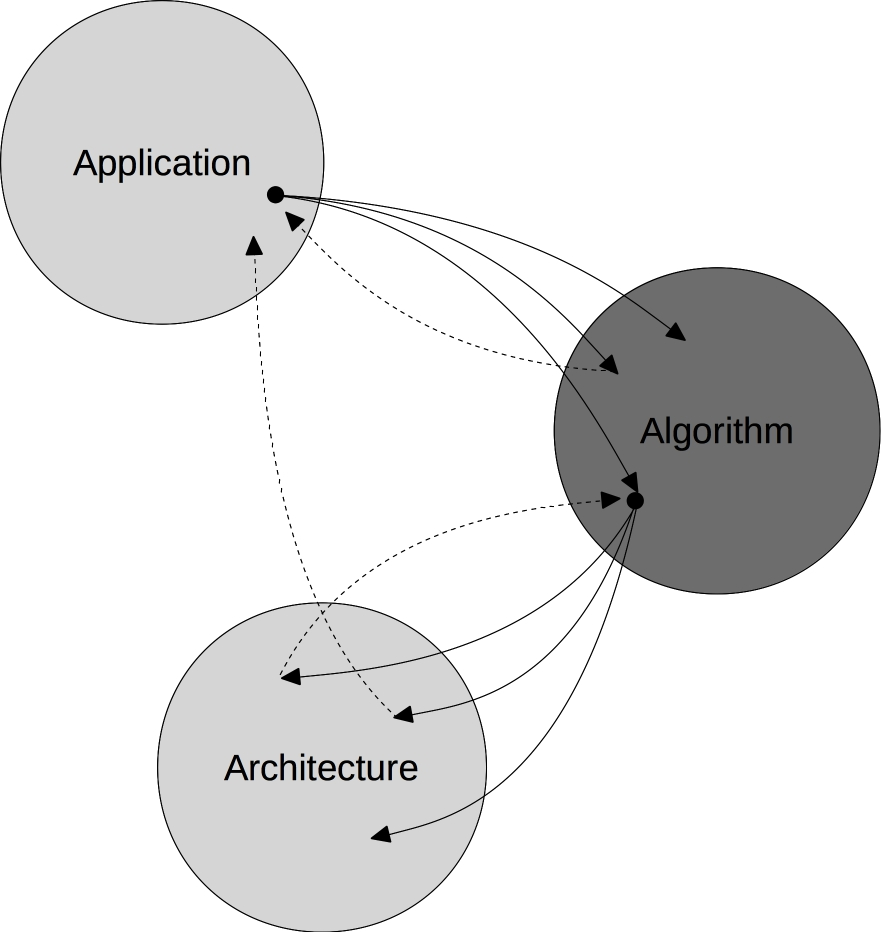
\includegraphics[scale=0.25]{figures/a3alg}
  \caption{A$^3$ model with the algorithm domain marked}
  \label{fig:a3alg}
\end{figure}

After the application analysis, a search for a fitting stereo vision algorithm can begin. During an internship at HSA systems a standard normalized cross-correlation (NCC) stereo matching algorithm was developed. An issue with the NCC algorithm is that it is not accurate near edges resulting in false matching around edges. For this project HSA systems wishes to find an algorithm which can be fast and is edge preserving. After some research two algorithms were found. These algorithms are \textit{Efficient Edge Preserving Stereo Matching} and \textit{Fast Cost-Volume Matching}. The description of these algorithm comes from \cite{cciugla2011efficient} and \cite{hosni2013fast}. The pseudo code for the EEPSM is created by the author while the FCV pseudo code comes from \cite{he2013guided} with some details added by the author of this thesis.
\section{Efficient Edge Preserving Stereo Matching (EEPSM):}\label{sec:eespm}
This algorithm is described in \cite{cciugla2011efficient}. This algorithm first calculates a cost for each pixel and disparity. This cost is a combination of the sum of absolute differences (SAD) and hamming distance of the census transform around each pixel. First the SAD is calculated:
\begin{flalign}
&& C^{SAD}_d(x,y) &=  \sum^3_{i=1}| I_{left}(x,y,i) - I_{right}(x+d,y,i) |  &&\label{eq:eepsmSAD}\\
\end{flalign}
where $i$ is the color (either red, green, or blue), $I_{left}(x,y,i)$ is a pixel in the left image or the reference image, and $I_{right}(x+d,y,i)$ is a pixel shifted by the disparity, $d$, in the right image or the target image.\\
It is noticed that this cost only uses the differences in color in a single pixel from each image and not a window around the pixel. Next the cost for a census transform is calculated.
\begin{flalign}
&& C^{CENSUS}_d(x,y) &= Ham(CT_{left}(x,y),CT_{right}(x+d,y)) && \\
\end{flalign}
Where $Ham(x_1,x_2)$ is the hamming distance between two bit strings and $CT(x,y)$ is the census transform around the pixel at $x,y$ for either the left image or the right image. The census transform converts the pixels in window around a center pixel into a bit string. Figure \vref{fig:census} shows a 3$\times$3 census transformer. If the intensity (grayscale value) of a pixel is higher than the center then it is converted to 1 and 0 otherwise and then bits are inserted into a bit string. \\
\begin{figure}[ht!]
  \centering
  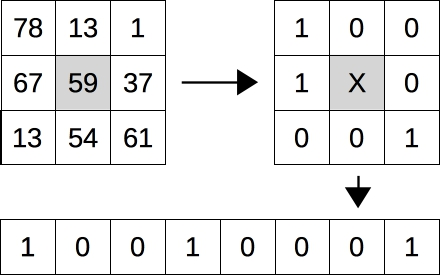
\includegraphics[height=3cm]{figures/census}
  \caption{Illustration of census transform}
  \label{fig:census}
\end{figure}

When the two cost values are calculated then they can be combined to a single cost value.
\begin{flalign}
&& C_d(x,y) &= \alpha \cdot C_d^{SAD} (x,y) + (1-\alpha)\cdot C^{CENSUS}_d (x,y) &&\label{eq:eepsmcost}
\end{flalign}
With the cost calculated the next step in the algorithm is to aggregate the cost. This is done in 3 steps. First step is to calculate permeability weights. Permeability is known from bio-medicine and describes the ability to transfer molecules through a cell membrane. The permeability weights are inspired by this and describes how well the color transfers from one pixel to another pixel and is expressed as:
\begin{flalign}
  && \mu(x,y) &= \min(e^{\frac{-\Delta R}{\sigma}},e^{\frac{-\Delta G}{\sigma}},e^{\frac{-\Delta B}{\sigma}}) &&\label{eq:premeability}
\end{flalign}
Where $\Delta R$, $\Delta G$, and $\Delta B$ is the difference in the specified color between two neighboring pixels and $\sigma$ is a smoothing factor. \\
The permeability weights should be calculated for each direction: up, down, left, and right and an example of the permeability of the downwards direction is shown in equation \vref{eq:permedown}
\begin{flalign}
  && \mu_{D}(x,y) &= \min(e^{\frac{-(R(x,y)-R(x,y-1))}{\sigma}},e^{\frac{-(G(x,y)-G(x,y-1))}{\sigma}},e^{\frac{-(B(x,y)-B(x,y-1))}{\sigma}}) && \label{eq:permedown}
\end{flalign}

The next step is to aggregate the cost in equation \vref{eq:eepsmcost} horizontally and this is achieved by using successive weighted summation (SWS) of the cost values along the left and right direction. The weights used in this summation will be the permeability weights for the right and left directions. The SWS for the right direction is expressed as:
\begin{flalign}
  && C^{R}_d (x) &= C_d(x)+ \mu_R (x-1) C^{R}_d (x-1) &&\label{eq:eepsmupdateR}\\
  && C^{R}_d (x) &= C_d(x)+ \sum_{i=1}^{x-1} \left(C_d(x-i)  \prod_{j=i}^{i} \mu_{R}(x-j) \right) &&\label{eq:eepsmupdateR2}
\end{flalign}
From equation \vref{eq:eepsmupdateR2} it is noticed that the cost, $C^R_d(x)$, will be affected by cost values from pixels to the left of point $x$ but the permeability weight ensures that the only pixel close to point $x$ and with similar color will have a large influence. When there are large changes in color it is assumed that the pixels will belong to a new object and therefore it ensures that only pixels from the same object have an influence on the cost. \\
When aggregating the right SWS the algorithm starts in the left side using equation \vref{eq:eepsmupdateR2} can be used as an update rule while moving in the right direction. A similar update rule exists for the left SWS. When the left SWS and the right SWS have been performed then these can be combined to a horizontal SWS:
\begin{flalign}
  && C^{H}_d (x) &= C_d(x)+ \mu_R (x-1) C^{R}_d (x-1) + \mu_L (x+1) C^{L}_d (x+1)&&\label{eq:eepsmupdatehorz}
\end{flalign}
When the horizontal aggregation have been completed then vertical aggregation can be performed. The vertical aggregation is similar to horizontal aggregation but instead of using the cost $C_d(x)$ it uses the cost from horizontal aggregation, $C^H_d (x)$, and moves in the vertical directions, up and down.\\

The cost from vertical aggregation, $C^V_d (x)$, will be influence by the cost from pixels belonging to the same object as pixel $x$ in greater or lesser degree. This cost can be used for minimization along disparity estimates with a winner take all approach. For occlusion perform a left-right cross check e.i. run the algorithm with the reference and target image changed around.

\subsubsection*{EEPSM psuedo code}
\textbf{Input:} \\
left image: $I_l$\\
right image: $I_r$\\
disparity estimate: $d$\\
\textbf{Output:} \\
filtering output: $q$\\
\textbf{Steps:}
\begin{enumerate}
  \item $C^{SAD}_d = f_{SAD}(I_l,I_{r,d})$\\
           $C^{CENSUS}_d = f_{Ham}(f_{CENSUS}(I_l),f_{CENSUS}(I_{r,d}))$
  \item $C_d = \alpha C^{SAD}_d + (1-\alpha) C^{CENSUS}_d$
  \item $\mu_D = f_{perme}(I_l,down)$ \\
           $\mu_U = f_{perme}(I_l,up)$ \\
           $\mu_L = f_{perme}(I_l,left)$ \\
           $\mu_R = f_{perme}(I_l,right)$
  \item $C^L = f_{SWS}(C_d,left)$\\
           $C^R = f_{SWS}(C_d,right)$
  \item $C^H = f_{SWS}(C^L,C^R,horizontal)$
  \item $C^U = f_{SWS}(C_d,up)$\\
           $C^D = f_{SWS}(C_d,down)$
  \item $C^V = f_{SWS}(C^U,C^D,vertical)$  
\end{enumerate}

\section{Fast Cost-Volume Matching (FCV):}
This algorithm is described in \cite{hosni2013fast}. 
As the algorithm in section \vref{sec:eespm} this algorithm calculates an initial cost and then aggregate this cost. The initial cost for this algorithm is also an combination of the sum of absolute differences and another cost. Instead of the cost based on census transform and hamming distance this algorithm uses difference in the gradient in the horizontal direction. The following equations shows the different cost function for this algorithm and equation \vref{eq:fcvinitcost} shows the combined initial cost. First the SAD cost is calculated and this equation is similar to equation \vref{eq:eepsmSAD}.\\
\begin{flalign}
 && C^{SAD}_{d} (x,y) &= \sum^3_{i=1}| I_{left}(x,y,i) - I_{right}(x+d,y,i) |  && \label{eq:fcvSAD}
\end{flalign}
Then the gradient cost is calculated.
\begin{flalign}
  && C^{Grad}_{d} (x,y) &= \nabla_x I_{left}^{g} (x,y) - \nabla_x I_{right}^{g} (x+d,y) &&
\end{flalign}
Where $\nabla_x$ is the gradient along the x-axis and $I_{left}^g$ and $I_{right}^g$ is the grayscale version of each image. When these cost values have been calculated they can be combined to a single cost value:
\begin{flalign}
  && C_{d} (x,y) &= \alpha \cdot C^{SAD}_{d} (x,y) + (1 - \alpha) \cdot C^{Grad}_{d} (x,y) &&\label{eq:fcvinitcost}
\end{flalign}
When the initial cost has been found it will be aggregated. The fast cost-volume algorithm will aggregate the cost values using a guided image filter. 
\begin{equation}
  C'_d (x_i,y_i) = \sum_{x_j,y_j} W_{(x_i,y_i),(x_j,y_j)}(I) C_d (x_j,y_j)
\end{equation}
Where $C'_d (x_i,y_i)$ is the aggregated cost in pixel $x_i,y_i$ with disparity estimate, $d$, $x_j,y_j$ is pixels in a square window around $x_i,y_i$, and $W_{(x_i,y_i),(x_j,y_j)}(I)$ is the filter weights based on a guidance image, $I$. Section \vref{sec:guidedif} will described how the filter weights are found.\\
This aggregate cost can then be used for minimization along the disparity estimates with a winner take all approach. For finding occlusion a left-right cross check will also be used here.
%\begin{flalign} \label{eq:fcvmin}
%  && f(x,y) &= \arg \min_{d \in [0,d_{max}]} C'_d(x,y)&&
%\end{flalign}

\subsection{Guided image filter} \label{sec:guidedif}
This filter is described in \cite{he2010guided} and \cite{he2013guided} and this section is mostly repeats what these articles describes.\\
To describe the guide image filter a standard linear translation-variant filtering process is defined:
\begin{equation}
  q_i = \sum_j W_{i,j}(I)p_j
\end{equation}
Where $i$ and $j$ are pixel indexes, $q$ the filter output, $W_{i,j}(I)$ is a filter kernel which is function of a guidance image $I$, and $p$ is a input image.\\

The guided image filter is defined as a linear model between a guidance image, $I$, and a filtering output, $q$:
\begin{equation}
  q_i = a_k I_i + b_k, \forall i \in \omega_k \label{eq:gif1}\\
\end{equation}
where $i$ and $k$ is pixel indexes, $\omega_k$ is a square window centered at $k$, and $a_k$ and $b_k$ is linear coefficients which are assumed to be constant in the window, $\omega_k$. \\
How to determine $a_k$ and $b_k$ is described in \cite{he2013guided} and the solution is shown in the following equations:
\begin{flalign}
  && a_k &= \dfrac{\frac{1}{|\omega|} \sum_{i \in \omega_k} I_i p_i - \mu_k \bar{p}_k}{\sigma^2_k + \epsilon} &&\label{eq:a_k}\\
  && b_k &= \bar{p}_k - a_k \mu_k && \label{eq:b_k}  
\end{flalign}
Where $|\omega|$ is the number of pixels in the window $\omega_k$, $\mu_k$ is the mean of $I$ in window $\omega_k$, $\bar{p}_k$ is the mean of input image $p$ in window $\omega_k$, $\sigma_k^2$ is the variance of $I$ in the window and $\epsilon$ is a regularization parameter which will penalize large $a_k$.\\

With $a_k$ and $b_k$ determined the filter output can be calculated:
\begin{equation}
  q_i = \frac{1}{|\omega|} \sum_{k|i \in \omega_k} (a_k I_i + b_k)
\end{equation}
$\sum_{k|i \in \omega_k} a_k = \sum_{k \in \omega_k} a_k$ because of symmetry in the square window and then the equation can be rewritten as
\begin{equation}
  q_i = \bar{a}_i I_i + \bar{b}_i
\end{equation}
Where $\bar{a}_i $ and $\bar{b}_i$ are the average coefficients for all windows that overlaps the pixel $i$ and are expressed as $\bar{a}_i = \frac{1}{|\omega|}\sum_{k \in \omega_k} a_k $ and $\bar{b}_i = \frac{1}{|\omega|}\sum_{k \in \omega_k} b_k$.\\

The guided image filter is used for its edge preserving property. The edge preserving property can be explained with the case where $I = p$ then:
\begin{flalign}
  && a_k &= \frac{\sigma_k^2}{\sigma_k^2 + \epsilon} &&\\
  && b_k &= (1-a_k)\mu_k &&
\end{flalign}
And if $\epsilon = 0$ then $a_k = 1$ and $b_k = 0$ but if $\epsilon > 0$ then two cases can occur. If the pixel is in an area where $I$ have a high variance in the window $\omega_k$ then $\sigma_k^2 \gg \epsilon$ and this results in $a_k \approx 1$ and $b_k \approx 0$. Instead if the pixel is in an area where $I$ is flat in the window $\omega_k$ then $\sigma_k^2 \ll \epsilon$ and this results in $a_k \approx 0$ and $b_k \approx 1$.\\
When these values are averaged then if the pixel are in a high variance area then the output is $q \approx p$ and if it instead is in a flat area the output is the average of surrounding pixels $q \approx p$.

\subsubsection*{FCV - grayscale - psuedo code}
\textbf{Input:} \\
left image: $I_l$\\
right image: $I_r$\\
disparity estimate: $d$\\
radius: $r$\\
epsilon: $\epsilon$\\
\textbf{Output:} \\
filtering output: $q$\\
\textbf{Steps:}
\begin{enumerate}
  \item $C^{SAD}_d = f_{SAD}(I_l,I_{r,d})$\\
           $C^{GRAD}_d = f_{GRAD}(I_l,I_{r,d})$
  \item $C_d = \alpha C^{SAD}_d + (1-\alpha) C^{GRAD}_d$
  \item $\mu_I = f_{mean}(I_l)$ \\
           $\mu_p = f_{mean}(C_d)$ \\
           $\rho_{II} = f_{mean}(I_l \cdot I_l)$ \\
           $\rho_{Ip} = f_{mean}(I_l \cdot C_d)$
  \item $\sigma_I = \rho_{II} - \mu_I \cdot \mu_I$\\
           $cov_{Ip} = \rho_{Ip} - \mu_I \cdot \mu_p$
  \item $a = cov_{Ip}/(\sigma_I + epsilon)$\\
           $b = \mu_p - a \cdot \mu_I $
  \item $\mu_a = f_{mean}(a)$\\
           $\mu_b = f_{mean}(b)$
  \item $q = \mu_a \cdot I_i + \mu_b$  
\end{enumerate}

The Guided image filter described in this chapter and therefore the FCV psuedo code is for a grayscale guidance image. For a color guidance image small changes have to be added. Equation \vref{eq} will then become:
\begin{equation}
  q_i = \textbf{a}_k^T \textbf{I}_i + b_k, \forall i \in \omega_k \label{eq:gif1}\\
\end{equation}
Where $\textbf{I}_i$ is a 3$\times$1 color vector and $\textbf{a}_k$ is 3$\times$1 coefficient vector. Then the guided image filter will be:
\begin{flalign}
  && \textbf{a}_k = (\Sigma_k + \epsilon U)&^{-1} \left(\frac{1}{|\omega|} \sum_{i \in \omega_k} \textbf{I}_i p_i - \mu_k \bar{p}_k \right) &&\label{eq:a_k}\\
  && b_k &= \bar{p}_k - \textbf{a}_k^T \mu_k && \label{eq:b_k}  \\
  && q_i &= \bar{\textbf{a}}_k^T \textbf{I}_i + \bar{b}_i&&
\end{flalign}
where $\sigma_k$ is the 3$\times$3 covariance matrix of $\textbf{I}$ in window, $\omega_k$ and $U$ is the 3$\times$3 identity matrix.
\subsubsection*{FCV - color - psuedo code}
\textbf{Input:} \\
left image: $I_l$\\
right image: $I_r$\\
disparity estimate: $d$\\
radius: $r$\\
epsilon: $\epsilon$\\
\textbf{Output:} \\
filtering output: $q$\\
\textbf{Steps:}
\begin{enumerate}
  \item $C^{SAD}_d = f_{SAD}(I_l,I_{r,d})$\\
           $C^{GRAD}_d = f_{GRAD}(I_l,I_{r,d})$
  \item $C_d = \alpha C^{SAD}_d + (1-\alpha) C^{GRAD}_d$
  \item $\mu_{I,r} = f_{mean}(I_{l,r})$ \\
           $\mu_{I,g} = f_{mean}(I_{l,g})$ \\
           $\mu_{I,b} = f_{mean}(I_{l,b})$ \\
           $\mu_p = f_{mean}(C_d)$ \\
           $\mu_{Ip,r} = f_{mean}(I_{l,r}\cdot p)$ \\
           $\mu_{Ip,g} = f_{mean}(I_{l,g}\cdot p)$ \\
           $\mu_{Ip,b} = f_{mean}(I_{l,b}\cdot p)$
  \item $\sigma_{I,r,r} = f_{mean}(I_{l,r}\cdot I_{l,r}) / N - \mu_{I,r} \cdot \mu_{I,r}$\\
           $\sigma_{I,r,g} = f_{mean}(I_{l,r}\cdot I_{l,g}) / N - \mu_{I,r} \cdot \mu_{I,g}$\\
           $\sigma_{I,r,b} = f_{mean}(I_{l,r}\cdot I_{l,b}) / N - \mu_{I,r} \cdot \mu_{I,b}$\\
           $\sigma_{I,g,g} = f_{mean}(I_{l,g}\cdot I_{l,g}) / N - \mu_{I,g} \cdot \mu_{I,g}$\\
           $\sigma_{I,g,b} = f_{mean}(I_{l,g}\cdot I_{l,b}) / N - \mu_{I,g} \cdot \mu_{I,b}$\\
           $\sigma_{I,b,b} = f_{mean}(I_{l,b}\cdot I_{l,b}) / N - \mu_{I,b} \cdot \mu_{I,b}$\\
           $cov_{Ip,r} = \mu_{Ip,r} - \mu_[I,r] \cdot \mu_p$\\
           $cov_{Ip,g} = \mu_{Ip,g} - \mu_[I,g] \cdot \mu_p$\\
           $cov_{Ip,b} = \mu_{Ip,b} - \mu_[I,b] \cdot \mu_p$
  \item $\Sigma = f_{\Sigma}(\sigma_{I,r,r},\sigma_{I,r,g},\sigma_{I,r,b},\sigma_{I,g,g},\sigma_{I,g,b},\sigma_{I,b,b})$\\
           $cov_{Ip}= [cov_{Ip,r}, cov_{Ip,g}, cov_{Ip,b}]$\\
           $a = cov_{Ip}\cdot f_{inv}(\sigma_I + epsilon\cdot U)$\\
           $b = \mu_p - a_r \cdot \mu_{I,r} - a_g \cdot \mu_{I,g} - a_b \cdot \mu_{I,b}$
  \item $\mu_{a,r} = f_{mean}(a_r)$\\
           $\mu_{a,g} = f_{mean}(a_g)$\\
           $\mu_{a,b} = f_{mean}(a_b)$\\
           $\mu_b = f_{mean}(b)$
  \item $q = \mu_{a,r} \cdot I_{i,r} +\mu_{a,g} \cdot I_{i,g}+\mu_{a,b} \cdot I_{i,b} + \mu_b$  
\end{enumerate}

\section{Simulation and comparison}\label{sec:simucomp}
With each algorithm described the algorithms have been implemented in Python for simulation and comparison. The code for FCV is inspired by example matlab code from \cite{hosni2013fast}. The code for EEPSM is written by the author of this thesis using the description in this chapter. None of the Python implementations have been optimized further.\\

The simulation were running on a MacBook Pro, Retina, 15-inch (mid 2015). This machine have the following specifications.
\begin{itemize}
  \item OS: OS X El Capitan - version 10.11.6
  \item Processor: Intel\copyright  Core$^{\text{TM}}$ i7-4770HQ
  \item Memory: 16 GB 1600 MHz DDR3
  \item Python version: 2.7.12 | Anaconda 2.5.0
  \item Relevant Python packages: Numpy v1.10.4, matplotlib v.1.5.1
\end{itemize}

For testing data sets from \cite{middlebury2016} is used. The stereo pairs are: Tsukuba, Cones, Teddy and Motorcycle and they are shown on figure \vref{fig:middlebury}. More information about the data sets is seen in appendix \vref{app:middlebury}.

\begin{figure}[ht]
  \centering
  \begin{subfigure}[t]{0.45\textwidth}
    \centering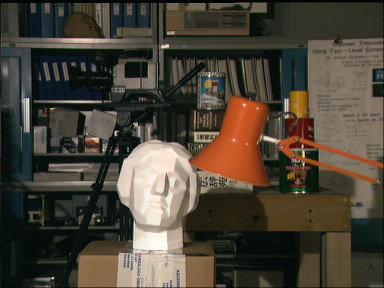
\includegraphics[height=5cm]{figures/tsul}
    \caption{Tsukuba \cite{Scharstein2002}\label{fig:tsu}}
  \end{subfigure}\hspace{0.5cm}
  \begin{subfigure}[t]{0.45\textwidth}
    \centering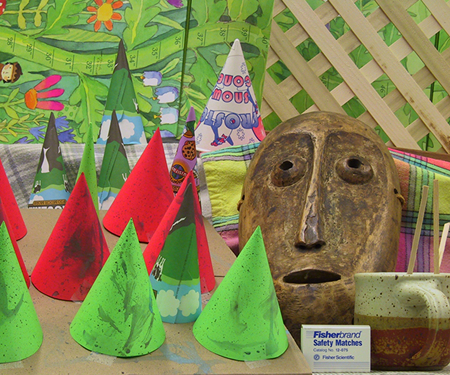
\includegraphics[height=5cm]{figures/conl}
    \caption{Cones \cite{Scharstein2003}\label{fig:cones}}
  \end{subfigure}
  \begin{subfigure}[t]{0.45\textwidth}
    \centering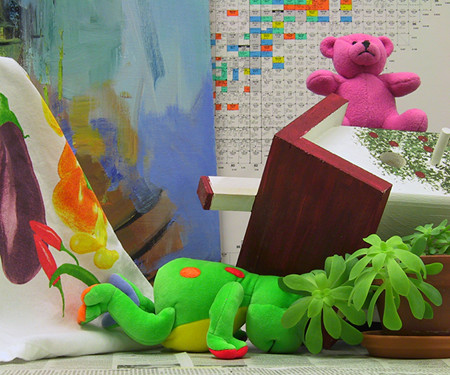
\includegraphics[height=5cm]{figures/tedl}
    \caption{Teddy \cite{Scharstein2003}\label{fig:ted}}
  \end{subfigure}\hspace{0.5cm}
  \begin{subfigure}[t]{0.45\textwidth}
    \centering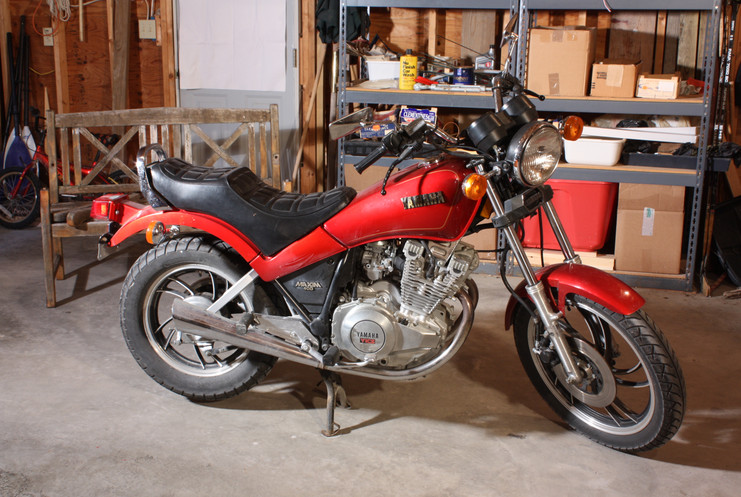
\includegraphics[height=5cm]{figures/motl}
    \caption{Motorcycle \cite{Scharstein2014}\label{fig:mot}}
  \end{subfigure}
  \caption{Middlebury data set - left images \cite{middlebury2016}\label{fig:middlebury}}
\end{figure}

\begin{table}[ht!]
  \centering
  \begin{tabular}{l c c c }
    \toprule
    Image & Resolution & EESPM & FCV \\
    \midrule
    Tsukuba & $384\times288$ & \SI{337}{\second}& \SI{180}{\second}\\
    Teddy & $450\times375$ & \SI{1147}{\second} & \SI{534}{\second} \\
    Cones & $450\times375$ & \SI{1105}{\second} & \SI{545}{\second} \\
    Motorcycle &  $741\times497$ & \SI{2471}{\second} & \SI{1378}{\second}\\
    \bottomrule
  \end{tabular}
  \caption{Run time for different stereo pairs \label{tab:runtime}}
\end{table}

\begin{table}[ht!]
  \centering
  \begin{tabular}{l c c c }
    \toprule
    Image & Resolution & EESPM & FCV \\
    \midrule
    Motorcycle & $741\times497$ & \SI{46}{\percent} & \SI{14}{\percent} \\
    \bottomrule
  \end{tabular}
  \caption{Procentage false disparity estimates \label{tab:falseesti}}
\end{table}

Figures \vref{fig:tsu_all} to \vref{fig:mot_all} shows resulting disparity maps.

\begin{figure}[ht]
  \centering
  \begin{subfigure}[t]{0.3\textwidth}
    \centering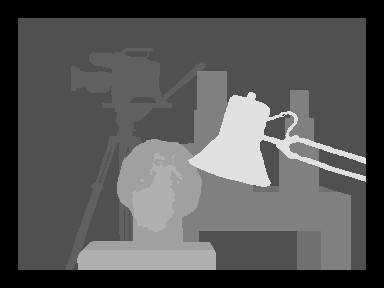
\includegraphics[width=5cm]{figures/tsu_gt}
    \caption{Ground truth \label{fig:tsu_gt}}
  \end{subfigure}\hspace{0.5cm}
  \begin{subfigure}[t]{0.3\textwidth}
    \centering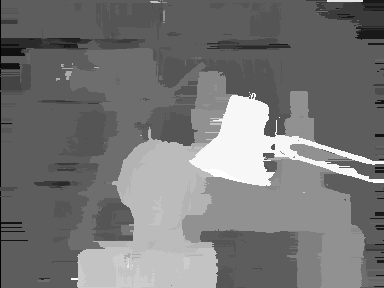
\includegraphics[width=5cm]{figures/tsu_fcv}
    \caption{FCV\label{fig:tsu_fcv}}
  \end{subfigure}\hspace{0.5cm}
  \begin{subfigure}[t]{0.3\textwidth}
    \centering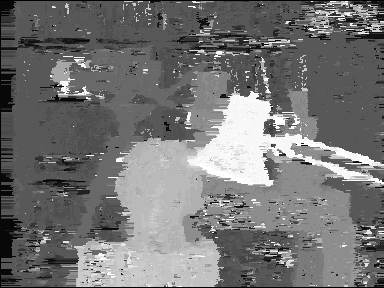
\includegraphics[width=5cm]{figures/tsu_eepsm1}
    \caption{EEPSM\label{fig:tsu_eepsm}}
  \end{subfigure}
  \caption{Tsukuba \cite{Scharstein2002}\label{fig:tsuall}}
\end{figure}

\begin{figure}[ht]
  \centering
  \begin{subfigure}[t]{0.3\textwidth}
    \centering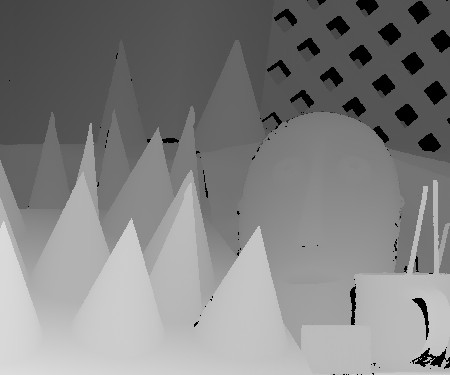
\includegraphics[width=5cm]{figures/con_gt}
    \caption{Ground truth \cite{Scharstein2003}\label{fig:con_gt}}
  \end{subfigure}\hspace{0.5cm}
  \begin{subfigure}[t]{0.3\textwidth}
    \centering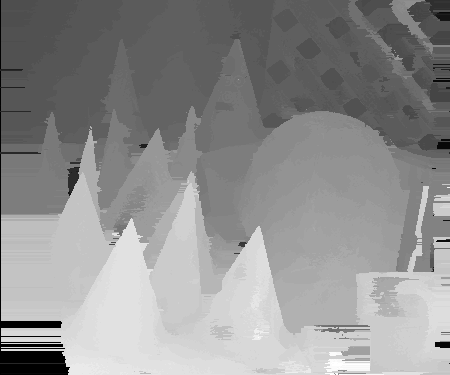
\includegraphics[width=5cm]{figures/con_fcv}
    \caption{FCV\label{fig:con_fcv}}
  \end{subfigure}\hspace{0.5cm}
  \begin{subfigure}[t]{0.3\textwidth}
    \centering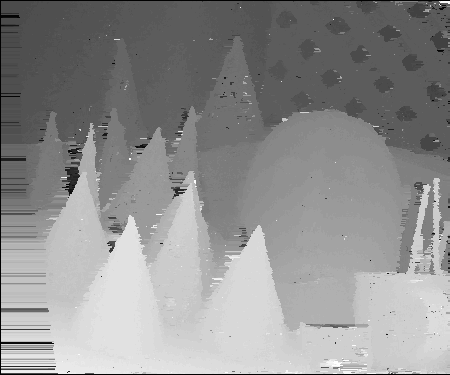
\includegraphics[width=5cm]{figures/con_eepsm1}
    \caption{EEPSM\label{fig:con_eepsm}}
  \end{subfigure}
  \caption{Cones \cite{Scharstein2003} \label{fig:conall}}
\end{figure}

\begin{figure}[ht]
  \centering
  \begin{subfigure}[t]{0.3\textwidth}
    \centering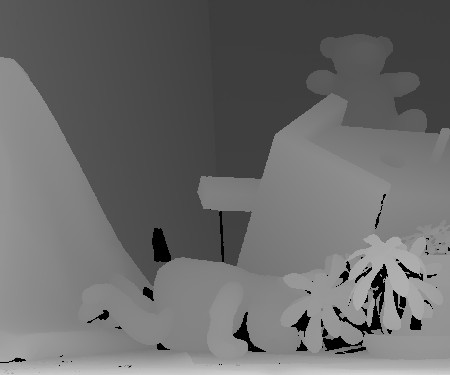
\includegraphics[width=5cm]{figures/ted_gt}
    \caption{Ground truth \cite{Scharstein2003}\label{fig:ted_gt}}
  \end{subfigure}\hspace{0.5cm}
  \begin{subfigure}[t]{0.3\textwidth}
    \centering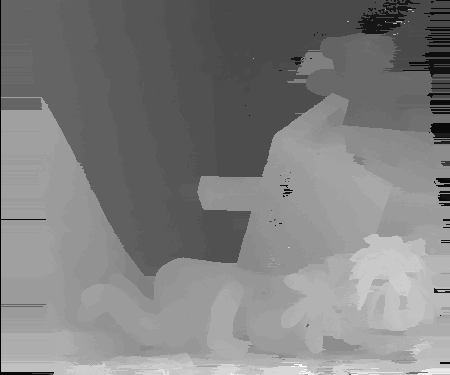
\includegraphics[width=5cm]{figures/ted_fcv}
    \caption{FCV\label{fig:ted_fcv}}
  \end{subfigure}\hspace{0.5cm}
  \begin{subfigure}[t]{0.3\textwidth}
    \centering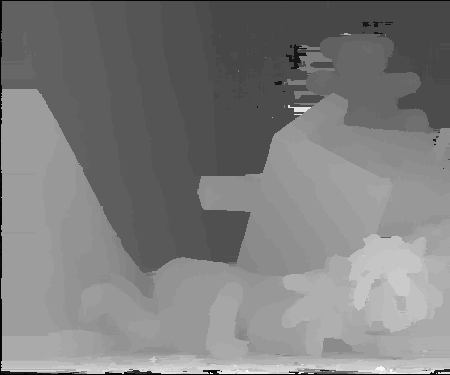
\includegraphics[width=5cm]{figures/ted_eepsm1}
    \caption{EEPSM\label{fig:ted_eepsm}}
  \end{subfigure}
  \caption{Teddy \cite{Scharstein2003} \label{fig:tedall}}
\end{figure}

\begin{figure}[ht]
  \centering
  \begin{subfigure}[t]{0.3\textwidth}
    \centering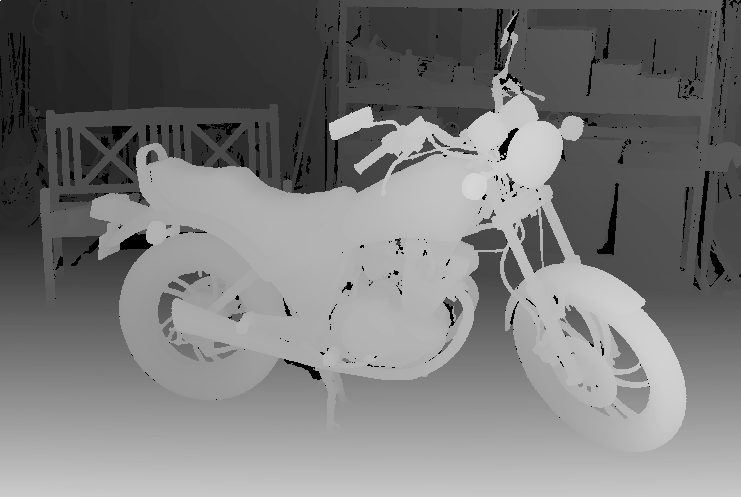
\includegraphics[width=5cm]{figures/mot_gt.png}
    \caption{Ground truth \cite{Scharstein2014} (Is dark due to scaling) \label{fig:mot_gt}}
  \end{subfigure}\hspace{0.5cm}
  \begin{subfigure}[t]{0.3\textwidth}
    \centering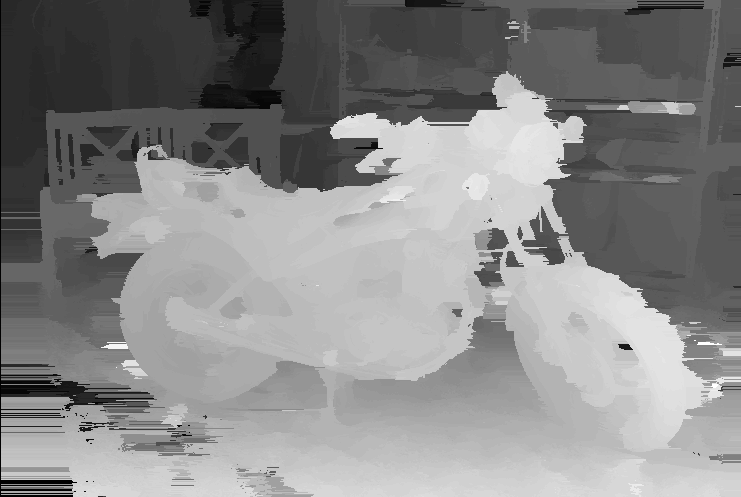
\includegraphics[width=5cm]{figures/mot_fcv}
    \caption{FCV\label{fig:mot_fcv}}
  \end{subfigure}\hspace{0.5cm}
  \begin{subfigure}[t]{0.3\textwidth}
    \centering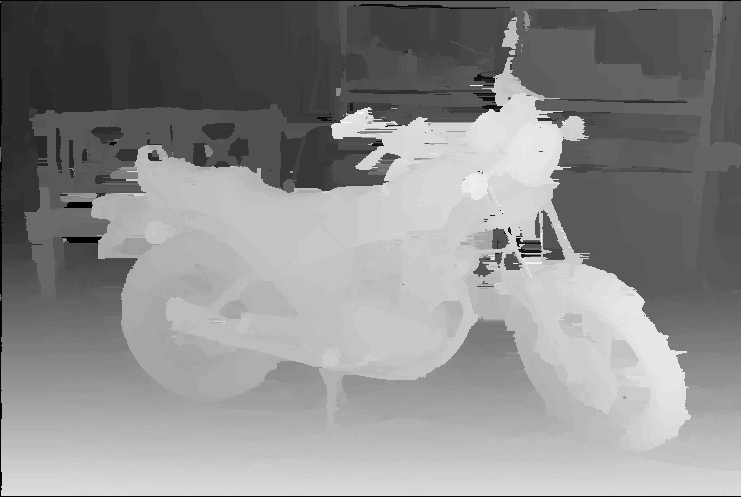
\includegraphics[width=5cm]{figures/mot_eepsm1}
    \caption{EEPSM\label{fig:mot_eepsm}}
  \end{subfigure}
  \caption{Motorcycle \cite{Scharstein2014}\label{fig:motall}}
\end{figure}

Looking at the Tsukuba test results on figure \vref{fig:tsuall} the FCV result seems better than the EEPSM result. FCV seems more smooth while EEPSM have a lot small areas with false matching. Both have a lot of vertical lines with false matching. Near the left border the errors from border occlusions is seen. These errors are worse in EEPSM compared to FCV.

Looking at the Cones test results on figure \vref{fig:conall} the FCV result seems more smooth than  the EEPSM result. The EEPSM is mostly smooth but noise is introduced in occluded areas. It is also noted that FCV doesn't handle the objects to right in the front whereas EEPSM have fewer false stere matches.

\section{Theoretical Complexity}
The simulations of the algorithms have to many unknown factors which can affect the performance e.g. the programmers knowledge of the algorithms and programming skills. To ensure a more precise?? estimation of the performance of the algorithms the theoretical complexity have been calculated. Table \vref{tb:theocompl} shows the number of addition, multiplications, divisions and comparisons used per pixel. It should be noted that the exponential function in the EEPSM algorithm have be approximated with a power series:
\begin{equation}
  e^x = \sum_{n=0}^{\infty} \dfrac{x^n}{n!} = 1 + x + \dfrac{x^2}{2!} + \dfrac{x^3}{3!} + \dots \label{eq:exppowser}
\end{equation}
Then it should be determined how many terms should be used for achieving sufficient precision. The exponential function is used in the calculation of permeability weights and the values all is in the interval $[-\dfrac{0}{25}; -\dfrac{255}{25}]$ 
\begin{table}[ht!]
  \centering
  \begin{tabular}{c c c c c c}
    \toprule
    & type & add/subtract & multiplication & division & comparisons \\
    \midrule
    EEPSM & C & $10320 \cdot N$ & $9340 \cdot N$ & $0$ & $6624 \cdot N$ \\
    & G & $8940 \cdot N$ & $4305 \cdot N$ & $0$ & $6624 \cdot N$ \\
    FCV & C & $268675 \cdot N$ & $57750 \cdot N$ & $275 \cdot N$ & $0$ \\
    & G & $95150 \cdot N$ & $14575 \cdot N$ & $275 \cdot N$ & $0$ \\
    \bottomrule
  \end{tabular}
  \caption{Complexity of each algorithm, where N is the number of pixels}
  \label{tb:theocompl}
\end{table}

I/O communication can also have a significant influence on the performance hence the memory usage for each algorithm have also been calculated and the result is shown in table \vref{tb:memuse}.
\begin{table}[ht!]
  \centering
  \begin{tabular}{c c c c c }
    \toprule
    & type & reads & writes & Memory $[$\si{\byte}$]$ \\
    \midrule
    EEPSM & C & $7751 \cdot N$ & $1375 \cdot N$ & $1381 \cdot N$ \\
    & G & $7189 \cdot N$ & $1375 \cdot N$ & $1377 \cdot N$ \\
    FCV & C & $22280 \cdot N$ & $275 \cdot N$ & $281 \cdot N$ \\
    & G & $11278 \cdot N$ & $275 \cdot N$ & $277 \cdot N$ \\
    \bottomrule
  \end{tabular}
  \caption{Memory resources used by each of the algorithms, where N is the number of pixels}
  \label{tb:memuse}
\end{table}

\section{Choosing an algorithm}
Not done\\
One of the algorithms described in this chapter should be chosen for further implementation on a FPGA. This choice is based on the results from section \vref{sec:simucomp}. Looking at table \ref{tab:runtime} it is seen that the Python implementation of the FCV algorithm has a far lower runtime than the EEPSM algorithm. The results might be misleading since the code for the FCV algorithm was inspired by an matlab example while the code for the EEPSM algorithm was written from the description.\\

Looking at table \vref{tab:falseesti} it is seen that the FCV algorithm is much better at matching than the EEPSM algorithm.\\

Referring to cost function described in chapter \vref{ch:req} it is noticed that time constraint and matching quality is the most important design metrics. This results in FCV to have a better estimated cost than EEPSM. From this the FCV algortihm is chosen.\\

It should also be noticed that the EEPSM algorithm requires a lot of memory since for aggregation of each pixel has to be kept saved in memory whereas the FCV algorithm can function like a running window. \\

Since the result for EEPSM is significantly worse than FCV it could indicate that the implementation of the EEPSM in python have errors but FCV is still chosen due to time constraint for the thesis. 

\section{Wrap-up}
Two edge preserving stereo vision algorithms have been described. The algorithms have been simulated using Python. The results shows that the FCV algorithm have a lower execution time and matches better than the EEPSM algorithm. But the results may indicate that the author have a better understanding of the FCV algorithm which gives this algorithm an edge. Regardless the FCV algorithm is chosen. 